% -*- root: ../main.tex -*-
%!TEX root = ../main.tex
% this file is called up by main.tex
% content in this file will be fed into the main document
% vim:textwidth=80 fo=cqt

In order  to successfully apply  any system identification technique,  the input
signal must be carefully  designed to be persistently exciting~\cite{Ljung1999}.
Narendra and Annaswamy~\cite{Narendra1984,Narendra1987}  were among the earliest
researchers  to provide  a detailed  treatment  of the  desirable properties  of
persistent excitation and their implication to the quality of the identification
output. A  practical method to achieve  persistent excitation is to  subject the
system under  consideration to  a sequence  of well-characterised  input signals
that  are  capable of  exciting  its  hypothesised  modes.  For this  task,  the
author  of this  thesis  chose  to use  the  data-quality  guidance provided  by
The~Mathworks~Inc.~\cite{mathworkssysid}\ and performed  an iterative refinement
until the identification procedure resulted in a generalisable model.

Before discussing the shape characteristics of the input sequence, its magnitude
must be established.  The various specially prepared input  sequence families do
not  share a  common definition  for their  magnitudes. A  guiding principle  in
system  identification is  that  it  is important  to  have  the input  signal's
magnitude  to  be  representative  of standard  operating  conditions.  Although
standardised  drive  cycle  profiles  are  available,  from  which  a  speed  to
current mapping  can be  performed, it  is impossible  to predict  a~priori, the
specific  amplitudes of  currents  that  the cell  may  undergo under  real-life
load  conditions.  Without  further  deterministic information,  the  author  of
this  thesis  chose to  interpret  magnitude  as  being  the peak  amplitude  of
the  input  current profile.  As  seen  in \cref{fig:uddssimp2dspmresults},  the
representative  \gls{udds}  drivecycle  input  profile  corresponds  to  a  peak
of~3C~\ie~\SI{180}{\ampere}.  Following   the  standard  principles   of  system
identification, it is desirable  for the inputs to the system  to lie along some
measure  of  central tendency.  This  is  to  enable  the identified  system  to
generalise well  \ie~not deviate too far  from the truth when  subject to inputs
that are far away from the central  measure. Yet another consideration is not to
saturate the identified model by choosing input magnitude to be too close to the
peak of  the expected  operating range. Taking  into account  all aforementioned
considerations,  the  peak amplitude  of  the  input  current  was fixed  at  2C
\ie~\ordfrac{2}{3} of the \gls{udds} profile's peak current amplitude.

\subsection{Training current profile}\label{subsec:trainingprofile}

Since not much prior  information is available about the poles  and zeros of the
electrolyte subsystem(s)  in question, a wide  variety of special waveforms  with a
sampling interval of \SI{1}{\second} were used for the current perturbation used
in this system identification task. The specific input sequence consisted of
\begin{enumerate}
    \item \gls{rbs}\quad (0--\SI{199}{\second})
    \item `Chirp' \ie~a swept cosine signal from 0--\SI{100}{\milli\hertz}\quad (200--\SI{799}{\second})
    \item Periodic \glsfmtlong{rbs} with a period of~\SI{200}{\second} and 2~such periods\quad (800--\SI{1199}{\second})
\end{enumerate}
thereby  helping  to  obtain  a  wide-sense  persistent  excitation.  The  swept
cosine  signal  is designed  to  excite  the low  frequency  (DC)  modes of  the
electrolyte subsystem and helps to capture the system's response to constant and
other systematically  varying input profiles.  The two \glspl{rbs}  are intended
to  target  the  poles  and  zeros  of  the  electrolyte  subsystem  that  would
typically be  excited by highly dynamic  input profiles. The periodicity  in one
of  the  \glspl{rbs} was  introduced  to  draw out  any  repeated  real pole  or
complex  conjugate  poles  poles  in  the system  that  might  otherwise  appear
to  be  a  single real  pole.  The  presence  of  both low  and  high  frequency
frequency  spectra in  the  combined  training set  presents  a  high degree  of
confidence to  capture the relevant  dynamics of the electrolyte  subsystem. The
input  current profile  used  for  this system  identification  task is  plotted
in \cref{fig:sysidtrainingcurrent}.

\begin{figure}[!htbp]
    \centering
    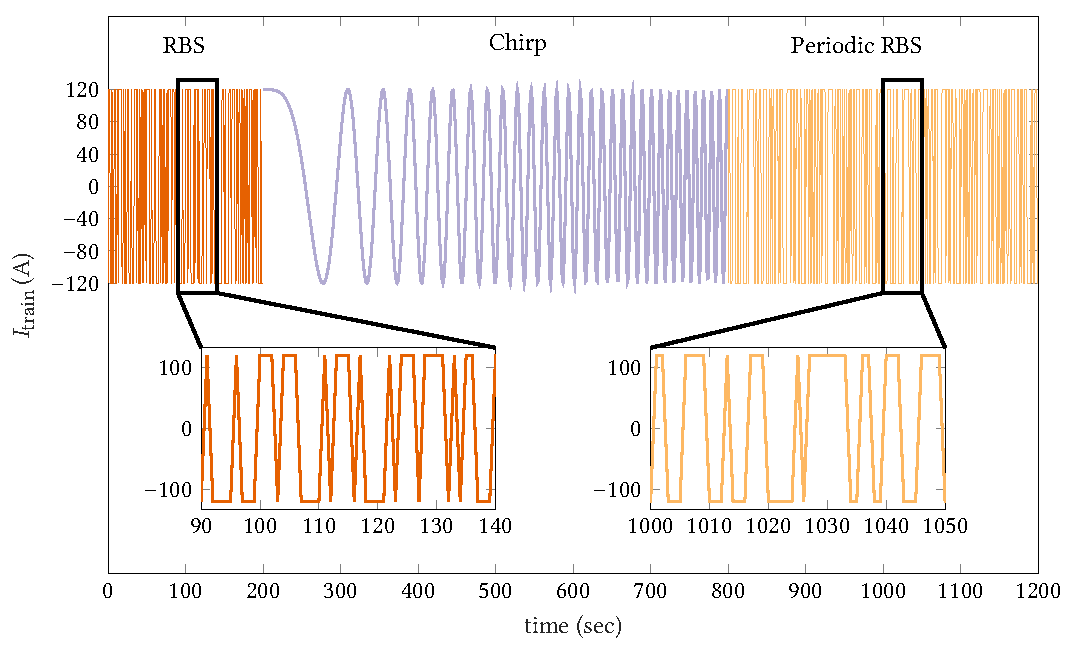
\includegraphics{sysid_train_input.pdf}
    \captionsetup{singlelinecheck=off}
    \caption[Input current profile used as the training set for system
    identification]{Input current profile used as the training set for system
    identification. The sequence consists of
    \begin{enumerate*}[label=\emph{\alph*})] \item a \glsfmtlong{rbs}, \item a
        chirp or swept cosine signal (0--\SI{100}{\milli\hertz}), and \item a periodic \glsfmtlong{rbs} \end{enumerate*} thereby
covering both low and high frequency spectra while incorporating the potential
to excite any periodic modes in the system to be identified.}
    \label{fig:sysidtrainingcurrent}
\end{figure}

\subsection{Validation current profile}

For the  purposes of identification,  the \gls{p2d}  model is considered  as the
true system. First, the current profile from  the training set is applied to the
\gls{p2d} model.  Its simulation results,  in particular the  numerically solved
concentration values  at each spatially  discretised node  in each of  the three
regions per time-step is integrated over the thickness of the respective regions
and multiplied with their respective porosities to obtain the number of moles of
\ch{Li^+} per unit area in each  of the three regions~$Q_{\text{e,}j}$. Only the
quantities  $Q_\text{e,n}$ and  $Q_\text{e,p}$  are chosen  as  the outputs  for
system  identification and  a  transfer  function model  is  fitted  as per  the
evaluation procedure discussed in \cref{sec:actualsysid}.

As with  any classical  curve fitting  (numerical regression)  procedure, system
identification is also  prone to overfitting the training data.  In general, the
`best' transfer  function that identifies the  given system is the  lowest order
model that not  only minimizes the training error, but  also minimizes the error
on a  previously unseen  validation dataset.  In the  absence of  an independent
validation  dataset,  the  training  error  can be  made  arbitrarily  small  by
increasing the number of poles and zeros of the transfer function models without
any bounds. However,  such a model shall not have  truly identified the dynamics
of the system  and shall not generalise well to  real-world datasets outside the
training realm. Hence, having an  independent validation current profile for the
task at hand is of paramount importance.

For the system identification task at  hand, the characteristic waveforms of the
validation profile were deliberately conjured to be differ vastly from that used
in training the model. The  validation profile consists of the following
sequence
\begin{enumerate}
    \item Periodic \gls{rgs} with 4~periods of \SI{200}{\second} each\quad (0--\SI{799}{\second})
    \item \gls{prbs} for emulating white noise \ie~with a flat power spectra
        across the frequency spectrum\quad (800--\SI{999}{\second})
    \item Multi-sine signal \ie~a signal consisting of sinusoids at
        various fundamental frequencies added together\quad (1000--\SI{1199}{\second})
\end{enumerate}

Overall,  the validation  profile has  been designed  to cover  a wide  range of
frequencies  akin to  the  training  profile, but  differing  completely in  its
time-domain appearance.  The specific  validation current  profile used  in this
system identification is shown in \cref{fig:sysidvalidationcurrent}.

\begin{figure}[!htbp]
    \centering
    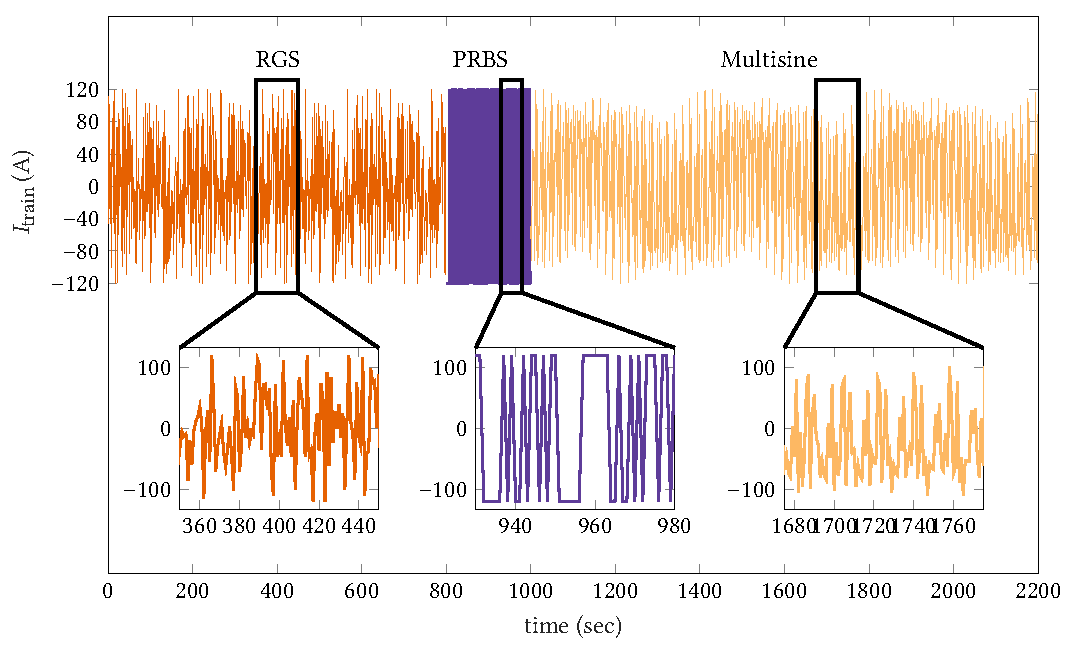
\includegraphics{sysid_validation_input.pdf}
    \captionsetup{singlelinecheck=off}
    \caption[Input current profile used as the validation set for system
    identification]{Input current profile used as the validation set for system
        identification. The sequence consists of
        \begin{enumerate*}[label=\emph{\alph*})]
            \item a \glsfmtlong{rgs},
            \item a \glsfmtlong{prbs}, and
            \item a multisine waveform
        \end{enumerate*}.
        The overall sequence  is intended to emulate the flat  power spectrum of
        white noise (with the \glsfmtshort{prbs}) and excite any poles and zeros
        within~\mbox{3$\sigma$} spread  of the  \glsfmtshort{rgs} mean.  The multisine
        signal is  swept is composed  of sinusoids with  fundamental frequencies
        from \SI{100}{\milli\hertz}  up to the Nyquist  frequency. Its amplitude
        variation  across the  frequency spectrum  increases the  probability to
        capture the  system's modes that  were possibly missed by  the preceding
        two waveforms.
    }%
    \label{fig:sysidvalidationcurrent}
\end{figure}

\textsc{MATLAB} code  that can be used  to generate the training  and validation
input profiles is shown in \cref{codesnippet:trainvalidsysidinput}.

\begin{listing}[!htbp]
\begin{minted}[mathescape,autogobble,bgcolor=mintedbg,escapeinside=||,texcomments=true]{matlab}
% Needs matlab's system identification toolbox
clear; close all; clc; format short g;
warning('off','Ident:dataprocess:idinput7'); % suppress sysid warnings
I_1C  = 60; % Amps
range = 2*[-I_1C I_1C]; % peak-peak swing is $\pm 2\text{C}=\SI{40}{\ampere}$
NumCh = 1; % no of channels (used by sysid toolbox for multichannel id)
Ts    = 1; % sampling interval

%% Random Binary Input Signal (RBS)
N  = 200; % samples per quantum of each waveform
u1 = idinput(N,'rbs',[],range); % 'idinput' from sysid toolbox
%% Chirp Signal (swept cosine)
t_chirp_start = 0;
t_chirp_end   = 3*N*Ts; %
t             = linspace(t_chirp_start,t_chirp_end,3*N);
f0            = 0;
f1            = 1e-1; % $f_1 = \SI{100}{\milli\hertz}$ is the max chirp frequency
u2            = max(range)*chirp(t,f0,t(end),f1)';
%% Periodic Random Binary Input Signal (Periodic RBS)
bin_seq_Period   = N; % seconds
bin_seq_Period_N = ceil(bin_seq_Period/Ts); % samples
bin_NumPeriod    = 2;
u3 = idinput([bin_seq_Period_N,NumCh,bin_NumPeriod],'rbs',[],range);
%% Random Guassian Signal (RGS)
rgs_Period         = N; % seconds
rgs_Period_samples = ceil(rgs_Period/Ts);
rgs_NumPeriod      = 4;
u4 = idinput([rgs_Period_samples,NumCh,rgs_NumPeriod],'rgs',[],range/2);
%% PseudoRandom Binary Signal (PRBS)
prbs_Period         = N; % seconds
prbs_Period_samples = ceil(prbs_Period/Ts);
u5                  = idinput(N,'prbs',[],range);
%% Multisine signal (sum of sines)
samples_per_Period = 2*N;
NumPeriod          = 3;
[u6,freq] = idinput([samples_per_Period 1 NumPeriod],'sine',[],range);

%% Split into training and validation data sets
I_load_train    = [u1;u2;u3];
I_load_validate = [u4;u5;u6];
\end{minted}
\caption{Generation of training and validation input current profiles in
\textsc{MATLAB}}
\label{codesnippet:trainvalidsysidinput}
\end{listing}
